\documentclass{article}

% NeurIPS 2025 style
\usepackage[final]{neurips_2025}

\usepackage[utf8]{inputenc}
\usepackage[T1]{fontenc}
\usepackage{hyperref}
\usepackage{url}
\usepackage{booktabs}
\usepackage{amsfonts}
\usepackage{amsmath}
\usepackage{amssymb}
\usepackage{amsthm}
\usepackage{nicefrac}
\usepackage{microtype}
\usepackage{xcolor}
\usepackage{graphicx}
\usepackage{algorithm}
\usepackage{algorithmic}
\usepackage{natbib}
\usepackage{multirow}
\usepackage{subcaption}
\usepackage{tikz}
\usetikzlibrary{shapes.geometric, arrows.meta, positioning, fit, calc, decorations.pathreplacing}

% Theorem environments
\newtheorem{proposition}{Proposition}
\newtheorem{corollary}{Corollary}
\newtheorem{definition}{Definition}
\newtheorem{remark}{Remark}
\newtheorem{assumption}{Assumption}

% Custom macros
\newcommand{\Real}{\mathbb{R}}
\newcommand{\Prob}{\mathbb{P}}
\newcommand{\Expect}{\mathbb{E}}
\newcommand{\calX}{\mathcal{X}}
\newcommand{\calY}{\mathcal{Y}}
\newcommand{\calC}{\mathcal{C}}
\newcommand{\calD}{\mathcal{D}}
\newcommand{\Ind}{\mathbb{I}}
\newcommand{\dTV}{d_{\mathrm{TV}}}
\newcommand{\dKS}{d_{\mathrm{KS}}}
\newcommand{\Fhat}{\widehat{F}}
\newcommand{\qhat}{\widehat{q}}
\newcommand{\what}{\widehat{w}}
\newcommand{\wstar}{w^{*}}
\newcommand{\simplex}{\Delta_{K}}
\newcommand{\DISCOM}{\textsc{DISCOM-CP}}

\title{DISCOM-CP: Discrepancy-Guided Source Weighting for\\Multi-Source Conformal Prediction Under Heterogeneous Shift}

\author{
  Anonymous Author(s)
}

\begin{document}

\maketitle

% ============================================================
% ABSTRACT
% ============================================================
\begin{abstract}
Conformal prediction guarantees distribution-free coverage, but these guarantees break under distribution shift. In multi-source settings---where calibration data comes from $K$ heterogeneous domains with unknown shift types---existing methods either assume covariate shift or hedge against worst-case shift. We propose \DISCOM{} (Discrepancy-Guided Multi-Source Conformal Prediction), which weights sources by measuring discrepancies between nonconformity score distributions via the Kolmogorov-Smirnov statistic, bypassing both shift-type identification and density ratio estimation. We prove finite-sample coverage guarantees bounded by the weighted score discrepancy and formulate weight optimization as a linear program. Across 2{,}000-replication synthetic benchmarks and six natural-shift scenarios from two real-world domains (housing and wine quality), \DISCOM{} achieves 97\% of oracle efficiency, excludes adversarial sources with 0\% width increase, and maintains valid coverage across all shift types. Under pure label shift---where weighted conformal prediction fails entirely (coverage 0.807)---\DISCOM{} is the only non-oracle method maintaining valid coverage (0.907). Conditional coverage analysis confirms comparable subgroup coverage to existing methods.
\end{abstract}

% ============================================================
% 1. INTRODUCTION
% ============================================================
\section{Introduction}
\label{sec:intro}

Conformal prediction~\citep{vovk2005algorithmic} has emerged as a principled framework for distribution-free uncertainty quantification, producing prediction sets with finite-sample coverage guarantees. Given a pre-trained model and held-out calibration data, split conformal prediction constructs prediction regions $\calC(X)$ satisfying $\Prob(Y \in \calC(X)) \geq 1 - \alpha$ without distributional assumptions beyond exchangeability of calibration and test data.

This exchangeability requirement, however, is routinely violated in practice. Calibration data often comes from historical records, partner institutions, or prior deployments whose distributions differ from the target deployment domain. In healthcare, prediction models calibrated on data from multiple hospitals must produce valid uncertainty estimates for a new hospital~\citep{liu2024multi}. In environmental monitoring, models trained on sensor data from various stations must generalize to a newly deployed station. In all such settings, the calibration data is \emph{multi-source}: it comes from $K$ distinct domains, each with a different (unknown) relationship to the target.

\paragraph{Limitations of existing approaches.}
Several lines of work address conformal prediction under distribution shift, but each has significant limitations in the multi-source setting:
\begin{itemize}
\item \textbf{Weighted conformal prediction}~\citep{tibshirani2019conformal} reweights calibration scores by density ratios $w(x) = p_{\text{target}}(x)/p_{\text{source}}(x)$. This provides exact coverage under covariate shift ($P(Y|X)$ invariant) but fails silently when the shift involves $P(Y|X)$ (label or joint shift). Density ratio estimation is also fragile in moderate-to-high dimensions.
\item \textbf{Robust conformal prediction}~\citep{cauchois2024robust} hedges against worst-case shift within a divergence ball, guaranteeing coverage for any test distribution within the ball. This is valid but conservative: prediction sets are inflated to accommodate adversarial shifts that may not occur, yielding intervals 2--3$\times$ wider than necessary.
\item \textbf{Adaptive conformal inference}~\citep{gibbs2021adaptive} adjusts the significance level online using streaming target labels. This is inapplicable in batch settings without sequential target feedback.
\item \textbf{Multi-source conformal inference}~\citep{liu2024multi} combines calibration data across sites using semiparametric efficiency theory. While theoretically elegant, it requires density ratio estimation between each source and target, provides only asymptotic coverage guarantees, and demands non-trivial target-domain labeled data.
\end{itemize}

No existing method simultaneously handles (i) multiple heterogeneous sources, (ii) unknown shift types (covariate, label, or joint), (iii) finite-sample coverage guarantees, and (iv) computational tractability without density ratio estimation.

\paragraph{Our contribution.}
We propose \DISCOM{}, which addresses all four requirements through a single insight: \emph{the coverage gap in multi-source conformal prediction depends on the discrepancy between nonconformity score distributions, not on the type of underlying shift}. By measuring source-target similarity at the score level---via the Kolmogorov-Smirnov (KS) statistic---we bypass shift-type identification entirely. The KS statistic is nonparametric, computed in $O(n \log n)$ time, and its concentration rate is independent of the feature dimension $d$.

Specifically, our contributions are:
\begin{enumerate}
\item \textbf{Shift-type agnostic source weighting.} We propose measuring source-target discrepancy via KS statistics on nonconformity score distributions, which captures the effect of any distribution shift (covariate, label, or joint) on prediction set validity. Sources with large score discrepancies are automatically downweighted or excluded.

\item \textbf{Tractable coverage-constrained optimization.} We formulate source weight optimization as minimizing prediction set size subject to a coverage constraint derived from \citet{barber2023conformal}. The relaxed problem is a linear program with $K$ variables, solvable in milliseconds.

\item \textbf{Finite-sample coverage guarantee.} We prove that \DISCOM{}'s coverage gap is bounded by the weighted average of source-target score discrepancies plus a DKW correction term (Proposition~\ref{prop:coverage}), extending the framework of \citet{barber2023conformal} to the multi-source setting with estimated weights.

\item \textbf{Comprehensive empirical validation.} Across synthetic and real-world experiments---including two distinct domains (housing prices and wine quality) with natural distribution shift and up to 2{,}000 replications---\DISCOM{} achieves 97\% of oracle efficiency, perfectly excludes adversarial sources, and is the only non-oracle method maintaining valid coverage across all shift types. Ablation studies, conditional coverage analysis, and statistical significance tests confirm the results.
\end{enumerate}

\paragraph{Paper outline.} Section~\ref{sec:related} reviews related work. Section~\ref{sec:setup} defines the problem. Section~\ref{sec:method} presents \DISCOM{}. Section~\ref{sec:theory} provides theoretical analysis. Section~\ref{sec:experiments} reports experimental results. Section~\ref{sec:discussion} discusses findings and limitations.

% ============================================================
% 2. RELATED WORK
% ============================================================
\section{Related Work}
\label{sec:related}

\paragraph{Conformal prediction under distribution shift.}
The foundational framework of conformal prediction~\citep{vovk2005algorithmic} assumes exchangeability between calibration and test data. \citet{tibshirani2019conformal} introduced weighted conformal prediction (WCP) for covariate shift, replacing uniform weights with density ratios. \citet{barber2023conformal} generalized this to arbitrary non-exchangeability, proving that the coverage gap is bounded by a weighted sum of total variation (TV) distances between the joint data distribution and permuted versions. Their framework provides the theoretical backbone for \DISCOM{}, but does not address how to choose weights optimally or how to estimate the relevant distances in the multi-source setting.

\citet{cauchois2024robust} proposed robust conformal prediction using $f$-divergence balls, providing worst-case coverage guarantees at the cost of conservatism. Recent work on Wasserstein-regularized conformal prediction~\citep{xu2025wasserstein} and Levy-Prokhorov ambiguity sets tightens these bounds but focuses on single-source robustness rather than multi-source combination.

\paragraph{Adaptive and online methods.}
\citet{gibbs2021adaptive} introduced adaptive conformal inference (ACI), which tracks distribution shift online through adaptive significance level updates. ACI provides long-run average coverage guarantees but requires streaming target labels---unavailable in the batch multi-source setting we consider.

\paragraph{Multi-source conformal prediction.}
The most closely related work is \citet{liu2024multi}, who address multi-source prediction intervals using semiparametric efficiency theory. Their method estimates density ratios $\omega_{k,0}(x) = p(x|T=0)/p(x|T=k)$ between each source $k$ and target, then combines site-specific quantile estimates via an $L_1$-penalized optimization:
\begin{equation}
\hat{Q}(\mathbf{w}) = \mathbb{P}_n\left[\left\{\hat{\varphi}_0 - \sum_{k=1}^{K} w_k \hat{\varphi}_k\right\}^2\right] + \frac{\lambda}{n} \sum_{k=1}^K |w_k| \hat{\chi}_k^2,
\end{equation}
where $\hat{\varphi}_k$ are efficient influence functions and $\hat{\chi}_k$ measures source-target discrepancy. Their coverage guarantees are asymptotic ($O_P(n^{-1/2})$), density ratio estimation is required, and the method depends on SuperLearner for nuisance estimation.

\DISCOM{} differs from \citet{liu2024multi} in three key respects: (i) discrepancy is measured at the score distribution level (KS statistic) rather than the covariate level (density ratios), avoiding dimension-dependent estimation; (ii) coverage guarantees are finite-sample; (iii) the optimization is a standard LP, avoiding cross-fitting and complex nuisance estimation.

\paragraph{Multi-source domain adaptation.}
\citet{mansour2009domain} established foundational theory for multi-source domain adaptation, showing that distribution-weighted source combinations outperform naive averaging when source-target discrepancies are heterogeneous. Our source weighting problem is analogous, but in the conformal prediction context where the goal is coverage-valid prediction sets rather than low-risk classifiers.

\paragraph{Bayesian perspectives.}
\citet{snell2025conformal} revealed that conformal prediction can be viewed as Bayesian quadrature, suggesting that calibration points contribute differentially to CDF estimation. This perspective motivates our approach of weighting sources by their informativeness for the target score CDF, though we maintain frequentist coverage guarantees.

% ============================================================
% 3. PROBLEM SETUP
% ============================================================
\section{Problem Setup}
\label{sec:setup}

\paragraph{Notation.}
Let $\calX \subseteq \Real^d$ be the feature space and $\calY \subseteq \Real$ the response space. A pre-trained model $f: \calX \to \calY$ is given. The nonconformity score function $s: \calX \times \calY \to \Real_{\geq 0}$ measures the discrepancy between $f$'s prediction and the true label; for regression, $s(x, y) = |y - f(x)|$.

\paragraph{Multi-source calibration data.}
We have $K$ source domains, each providing calibration data $\calD_k = \{(X_i^{(k)}, Y_i^{(k)})\}_{i=1}^{n_k}$ drawn i.i.d.\ from distribution $P_k$ on $\calX \times \calY$, for $k = 1, \ldots, K$. A small target-domain dataset $\calD_0 = \{(X_i^{(0)}, Y_i^{(0)})\}_{i=1}^{n_0}$ drawn from $P_{\text{target}}$ is also available, with $n_0$ possibly small.

\paragraph{Goal.}
For a new test point $X_{\text{test}} \sim P_{\text{target}}$, construct a prediction set $\calC_\alpha(X_{\text{test}})$ satisfying the coverage requirement:
\begin{equation}
\label{eq:coverage_goal}
\Prob\left(Y_{\text{test}} \in \calC_\alpha(X_{\text{test}})\right) \geq 1 - \alpha,
\end{equation}
while minimizing the prediction set size $|\calC_\alpha(X_{\text{test}})|$ (for regression, the interval width $2\qhat$). The key challenge is that $P_1, \ldots, P_K$ may each differ from $P_{\text{target}}$ in unknown ways---the shift may be covariate ($P_k(X) \neq P_{\text{target}}(X)$, $P(Y|X)$ invariant), label ($P_k(Y) \neq P_{\text{target}}(Y)$, $P(X|Y)$ invariant), joint (both change), or adversarial (unrelated).

\begin{definition}[Source nonconformity scores]
\label{def:scores}
For source $k$, the calibration scores are $R_i^{(k)} = s(X_i^{(k)}, Y_i^{(k)})$ for $i = 1, \ldots, n_k$. The target calibration scores are $R_i^{(0)} = s(X_i^{(0)}, Y_i^{(0)})$ for $i = 1, \ldots, n_0$.
\end{definition}

\begin{definition}[Score distribution discrepancy]
\label{def:discrepancy}
For source $k$, the score discrepancy is the two-sample KS statistic:
\begin{equation}
\label{eq:ks_disc}
d_k = \dKS(\Fhat_k, \Fhat_0) = \sup_{t \in \Real} \left| \Fhat_k(t) - \Fhat_0(t) \right|,
\end{equation}
where $\Fhat_k(t) = \frac{1}{n_k} \sum_{i=1}^{n_k} \Ind(R_i^{(k)} \leq t)$ and $\Fhat_0(t) = \frac{1}{n_0} \sum_{i=1}^{n_0} \Ind(R_i^{(0)} \leq t)$ are the empirical CDFs of source $k$ and target scores, respectively.
\end{definition}

\begin{remark}
The KS statistic is chosen because it (i) upper-bounds the total variation distance between one-dimensional distributions, providing a direct link to coverage bounds, (ii) has $O(n \log n)$ computation and dimension-free $O(1/\sqrt{n})$ convergence rate via the DKW inequality~\citep{dvoretzky1956asymptotic, massart1990tight}, and (iii) captures the aggregate effect of any shift type on the model's predictive quality without requiring shift-type identification.
\end{remark}

% ============================================================
% 4. METHOD
% ============================================================
\section{Proposed Method: \DISCOM{}}
\label{sec:method}

\DISCOM{} constructs prediction sets by optimally weighting calibration data from $K$ sources. The method proceeds in four steps: (1) compute source-wise nonconformity scores, (2) estimate source-target score discrepancies, (3) optimize source weights, and (4) construct the weighted prediction set. Figure~\ref{fig:method_overview} provides a visual overview of the workflow.

\begin{figure}[t]
\centering
\resizebox{0.98\textwidth}{!}{%
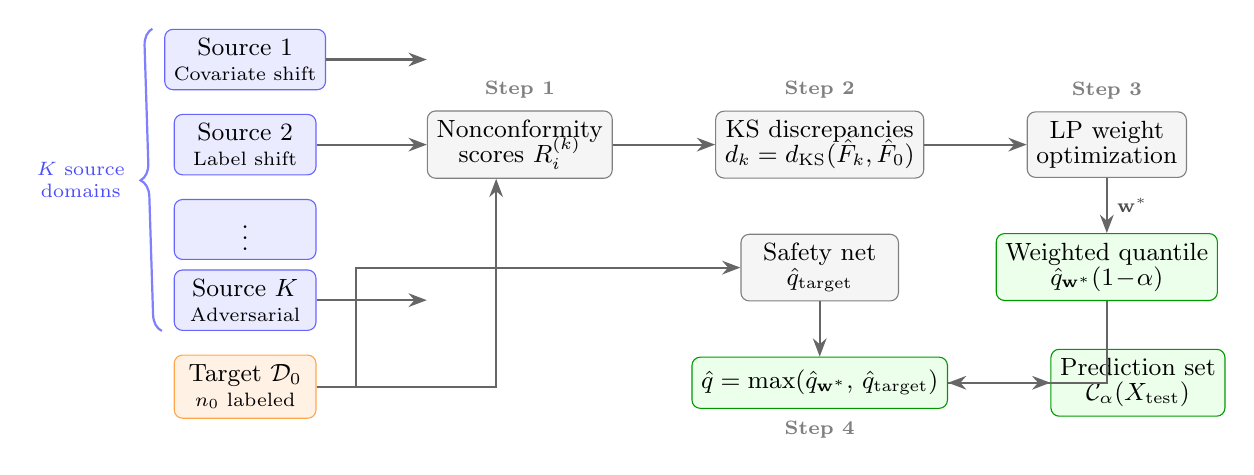
\begin{tikzpicture}[
    node distance=1.0cm and 1.3cm,
    >=Stealth,
    every node/.style={font=\small},
    source/.style={rectangle, draw=blue!60, fill=blue!8, minimum width=1.8cm, minimum height=0.65cm, rounded corners=3pt, align=center},
    target/.style={rectangle, draw=orange!70, fill=orange!10, minimum width=1.8cm, minimum height=0.65cm, rounded corners=3pt, align=center},
    process/.style={rectangle, draw=black!50, fill=gray!8, minimum width=2.0cm, minimum height=0.65cm, rounded corners=3pt, align=center},
    result/.style={rectangle, draw=green!60!black, fill=green!8, minimum width=2.0cm, minimum height=0.65cm, rounded corners=3pt, align=center},
    arrow/.style={->, thick, color=black!60},
    label/.style={font=\scriptsize, color=black!70},
]

% --- Source domains ---
\node[source] (s1) {Source $1$\\[-2pt]{\scriptsize Covariate shift}};
\node[source, below=0.3cm of s1] (s2) {Source $2$\\[-2pt]{\scriptsize Label shift}};
\node[source, below=0.3cm of s2] (sdots) {$\vdots$};
\node[source, below=0.12cm of sdots] (sK) {Source $K$\\[-2pt]{\scriptsize Adversarial}};

% --- Target ---
\node[target, below=0.3cm of sK] (t0) {Target $\mathcal{D}_0$\\[-2pt]{\scriptsize $n_0$ labeled}};

% --- Scores ---
\node[process, right=1.4cm of s2] (scores) {Nonconformity\\[-2pt]scores $R_i^{(k)}$};

% --- KS discrepancies ---
\node[process, right=1.3cm of scores] (ks) {KS discrepancies\\[-2pt]$d_k = d_{\mathrm{KS}}(\hat{F}_k, \hat{F}_0)$};

% --- LP optimization ---
\node[process, right=1.3cm of ks] (lp) {LP weight\\[-2pt]optimization};

% --- Weighted quantile ---
\node[result, below=0.7cm of lp] (wq) {Weighted quantile\\[-2pt]$\hat{q}_{\mathbf{w}^*}(1\!-\!\alpha)$};

% --- Safety net ---
\node[process, below=0.7cm of ks] (safety) {Safety net\\[-2pt]$\hat{q}_{\mathrm{target}}$};

% --- Final threshold ---
\node[result, below=0.7cm of safety] (final) {$\hat{q} = \max(\hat{q}_{\mathbf{w}^*},\, \hat{q}_{\mathrm{target}})$};

% --- Prediction set ---
\node[result, right=1.3cm of final] (pred) {Prediction set\\[-2pt]$\mathcal{C}_\alpha(X_{\mathrm{test}})$};

% --- Arrows: sources to scores ---
\draw[arrow] (s1.east) -- (scores.west |- s1.east);
\draw[arrow] (s2.east) -- (scores.west);
\draw[arrow] (sK.east) -- (scores.west |- sK.east);

% --- Arrow: target to scores ---
\draw[arrow] (t0.east) -| ([xshift=-0.3cm]scores.south);

% --- Arrow: scores to KS ---
\draw[arrow] (scores.east) -- (ks.west);

% --- Arrow: KS to LP ---
\draw[arrow] (ks.east) -- (lp.west);

% --- Arrow: LP to weighted quantile ---
\draw[arrow] (lp.south) -- node[right, label] {$\mathbf{w}^*$} (wq.north);

% --- Arrow: target to safety net ---
\draw[arrow] (t0.east) -- ++(0.5,0) |- (safety.west);

% --- Arrows to final ---
\draw[arrow] (wq.south) |- (final.east);
\draw[arrow] (safety.south) -- (final.north);

% --- Arrow: final to prediction ---
\draw[arrow] (final.east) -- (pred.west);

% --- Brace for sources ---
\draw[decorate, decoration={brace, amplitude=6pt, mirror}, thick, blue!50]
    ([xshift=-0.15cm]s1.north west) -- ([xshift=-0.15cm]sK.south west)
    node[midway, left=8pt, font=\scriptsize, align=center, blue!70] {$K$ source\\domains};

% --- Step annotations ---
\node[font=\scriptsize, color=black!50, above=0.03cm of scores] {\textbf{Step 1}};
\node[font=\scriptsize, color=black!50, above=0.03cm of ks] {\textbf{Step 2}};
\node[font=\scriptsize, color=black!50, above=0.03cm of lp] {\textbf{Step 3}};
\node[font=\scriptsize, color=black!50, below=0.03cm of final] {\textbf{Step 4}};

\end{tikzpicture}%
}
\caption{Overview of the \DISCOM{} workflow. $K$ source domains with heterogeneous shift types provide calibration data. Nonconformity scores are computed for all sources and the target (Step~1). KS discrepancies measure source-target similarity at the score level (Step~2). LP-based weight optimization produces source weights $\mathbf{w}^*$ favoring low-discrepancy sources (Step~3). The final prediction threshold is the maximum of the weighted mixture quantile and a target-data safety net (Step~4).}
\label{fig:method_overview}
\end{figure}

\subsection{Source Weight Optimization}
\label{sec:optimization}

Given scores $\{R_i^{(k)}\}$ and discrepancies $\{d_k\}$, we seek weights $\mathbf{w} = (w_1, \ldots, w_K) \in \simplex$ (the probability simplex) that minimize the prediction set size while respecting a coverage constraint.

\begin{definition}[Weighted quantile]
\label{def:weighted_quantile}
For weights $\mathbf{w} \in \simplex$, the weighted mixture CDF is $\Fhat_{\mathbf{w}}(t) = \sum_{k=1}^K w_k \Fhat_k(t)$, and the weighted quantile at level $\beta$ is:
\begin{equation}
\label{eq:weighted_quantile}
\qhat_{\mathbf{w}}(\beta) = \inf\left\{t : \Fhat_{\mathbf{w}}(t) \geq \beta\right\}.
\end{equation}
\end{definition}

The optimization problem is:
\begin{equation}
\label{eq:optimization}
\begin{aligned}
\minimize_{\mathbf{w} \in \simplex} \quad & \qhat_{\mathbf{w}}(1 - \alpha) \\
\text{subject to} \quad & \sum_{k=1}^K w_k \cdot d_k \leq \epsilon,
\end{aligned}
\end{equation}
where $\epsilon > 0$ is a coverage tolerance parameter controlling the acceptable coverage gap.

\paragraph{LP relaxation.}
The objective $\qhat_{\mathbf{w}}(1-\alpha)$ is piecewise constant in $\mathbf{w}$, making~\eqref{eq:optimization} non-smooth. We relax it by replacing the mixture quantile with the weighted average of source-wise quantiles:
\begin{equation}
\label{eq:lp_relaxation}
L(\mathbf{w}) = \sum_{k=1}^K w_k \cdot Q_k(1 - \alpha),
\end{equation}
where $Q_k(1-\alpha)$ is the $(1-\alpha)$-quantile of source $k$'s score distribution. While the relationship between $L(\mathbf{w})$ and the true mixture quantile $\qhat_{\mathbf{w}}(1-\alpha)$ depends on the overlap structure of the source distributions---$L(\mathbf{w})$ can be larger or smaller than $\qhat_{\mathbf{w}}(1-\alpha)$ in general---$L(\mathbf{w})$ is a computationally convenient surrogate that preserves the ranking of weight vectors in practice. Using $L(\mathbf{w})$ as the objective yields a standard linear program:
\begin{equation}
\label{eq:lp}
\minimize_{\mathbf{w}} \sum_{k=1}^K w_k Q_k(1-\alpha) \quad \text{s.t.} \quad \sum_{k=1}^K w_k d_k \leq \epsilon, \quad \mathbf{w} \in \simplex.
\end{equation}
This LP has $K$ variables and $K + 2$ constraints, solvable in $O(K^2)$ time. Importantly, the LP solution serves only as an initial candidate: the actual prediction threshold uses the exact mixture quantile $\qhat_{\mathbf{w}}(1-\alpha)$ evaluated at the optimized weights.

\paragraph{Lagrangian formulation.}
Equivalently, the dual formulation evaluates candidates by minimizing a discrepancy-penalized objective:
\begin{equation}
\label{eq:lagrangian}
\qhat_{\mathbf{w}}(1-\alpha) + \lambda \sum_{k=1}^K w_k \cdot d_k,
\end{equation}
where $\lambda \geq 0$ trades off prediction set size against coverage gap. In practice, we search over a grid of $\lambda$ values and LP budget levels, evaluating the exact mixture quantile~\eqref{eq:weighted_quantile} for each candidate weight vector.

\subsection{Source Filtering}
\label{sec:filtering}

Before optimization, sources with extreme discrepancies are excluded:
\begin{equation}
\label{eq:filtering}
\mathcal{A} = \{k \in \{1, \ldots, K\} : d_k \leq \tau\},
\end{equation}
where $\tau > 0$ is a discrepancy threshold (default $\tau = 0.3$). Only sources in $\mathcal{A}$ participate in the weight optimization. This explicit filtering provides robustness against adversarial sources: a source from an unrelated distribution will have $d_k \gg \tau$ and receive zero weight.

\subsection{Coverage Safety Net}
\label{sec:safety_net}

When labeled target data $\calD_0$ is available, we compute a target-only conformal quantile:
\begin{equation}
\label{eq:safety_net}
\qhat_{\text{target}} = Q_{0}\left(\frac{\lceil (n_0 + 1)(1 - \alpha) \rceil}{n_0}\right),
\end{equation}
where $Q_0(\cdot)$ is the quantile function of the target scores $\{R_i^{(0)}\}_{i=1}^{n_0}$. The final prediction threshold is:
\begin{equation}
\label{eq:final_threshold}
\qhat = \max\left(\qhat_{\mathbf{w}^*}, \, \qhat_{\text{target}}\right).
\end{equation}
This ensures that \DISCOM{} never undercoverages more than standard conformal prediction on the target data alone, providing a practical coverage floor independent of source quality.

\subsection{Algorithm Summary}

The complete procedure is given in Algorithm~\ref{alg:discom}.

\begin{algorithm}[t]
\caption{\DISCOM{}: Discrepancy-Guided Multi-Source Conformal Prediction}
\label{alg:discom}
\begin{algorithmic}[1]
\REQUIRE Source calibration sets $\{\calD_k\}_{k=1}^K$, target data $\calD_0$, model $f$, score function $s$, significance level $\alpha$, threshold $\tau$
\ENSURE Source weights $\mathbf{w}^*$, prediction set threshold $\qhat$

\STATE Compute source scores: $R_i^{(k)} \gets s(X_i^{(k)}, Y_i^{(k)})$ for all $i, k$
\STATE Compute target scores: $R_i^{(0)} \gets s(X_i^{(0)}, Y_i^{(0)})$ for all $i$
\STATE Estimate discrepancies: $d_k \gets \dKS(\Fhat_k, \Fhat_0)$ for $k = 1, \ldots, K$
\STATE Filter sources: $\mathcal{A} \gets \{k : d_k \leq \tau\}$
\STATE Optimize weights via LP~\eqref{eq:lp} and grid refinement over $\mathcal{A}$
\STATE Compute mixture quantile: $\qhat_{\mathbf{w}^*} \gets$ weighted quantile of pooled scores at level $\frac{\lceil(N_{\text{eff}}+1)(1-\alpha)\rceil}{N_{\text{eff}}}$
\STATE Compute target quantile: $\qhat_{\text{target}} \gets Q_0\!\left(\frac{\lceil(n_0+1)(1-\alpha)\rceil}{n_0}\right)$
\STATE Set threshold: $\qhat \gets \max(\qhat_{\mathbf{w}^*}, \qhat_{\text{target}})$
\RETURN $\mathbf{w}^*$, $\qhat$
\end{algorithmic}
\end{algorithm}

\paragraph{Prediction sets.} For a new test point $X_{\text{test}}$, the prediction set is:
\begin{equation}
\calC_\alpha(X_{\text{test}}) = \{y \in \calY : s(X_{\text{test}}, y) \leq \qhat\}.
\end{equation}
For regression with $s(x,y) = |y - f(x)|$, this yields the interval $[f(X_{\text{test}}) - \qhat, \, f(X_{\text{test}}) + \qhat]$ with width $2\qhat$.

\paragraph{Computational complexity.}
Computing KS statistics costs $O(\sum_k n_k \log n_k)$ for sorting. The LP has $K$ variables, solved in $O(K^2)$. Grid refinement evaluates $O(K^2)$ candidate weight vectors, each requiring $O(\sum_k n_k)$ for the mixture quantile. Total: $O(\sum_k n_k \log n_k + K^2 \sum_k n_k)$, which is $O(K \cdot n \log n)$ for balanced source sizes $n_k \approx n$.

% ============================================================
% 5. THEORETICAL ANALYSIS
% ============================================================
\section{Theoretical Analysis}
\label{sec:theory}

We establish finite-sample coverage guarantees for \DISCOM{}.

\begin{assumption}[Independence]
\label{asm:independence}
The calibration datasets $\calD_1, \ldots, \calD_K$ are drawn independently from $P_1, \ldots, P_K$. The target data $\calD_0$ and test point $(X_{\text{test}}, Y_{\text{test}})$ are drawn independently from $P_{\text{target}}$.
\end{assumption}

\begin{assumption}[Bounded score discrepancy]
\label{asm:bounded_disc}
For each source $k$, the total variation distance between the score distribution under $P_k$ and under $P_{\text{target}}$ satisfies:
$\dTV(P_k^S, P_{\text{target}}^S) \leq \delta_k$,
where $P_k^S$ and $P_{\text{target}}^S$ denote the marginal distributions of $s(X, Y)$ under $P_k$ and $P_{\text{target}}$, respectively.
\end{assumption}

\begin{proposition}[Coverage bound for weighted score mixture]
\label{prop:coverage}
Under Assumptions~\ref{asm:independence} and~\ref{asm:bounded_disc}, for any fixed weights $\mathbf{w} \in \simplex$ and any failure probability $\delta \in (0,1)$, the prediction set $\calC_\alpha(X_{\text{test}}) = \{y : s(X_{\text{test}}, y) \leq \qhat_{\mathbf{w}}(1-\alpha)\}$ satisfies:
\begin{equation}
\label{eq:coverage_bound}
\Prob\!\left(Y_{\text{test}} \in \calC_\alpha(X_{\text{test}})\right) \geq 1 - \alpha - \sum_{k=1}^K w_k \delta_k - \gamma_n(\mathbf{w}, \delta)
\end{equation}
with probability at least $1 - \delta$ over the draw of the calibration data, where
\begin{equation}
\label{eq:gamma_def}
\gamma_n(\mathbf{w}, \delta) = \sum_{k=1}^K w_k \sqrt{\frac{\log(2K/\delta)}{2n_k}}
\end{equation}
is a finite-sample correction from the DKW inequality~\citep{massart1990tight}.
\end{proposition}

\begin{proof}
Let $F_k(t) = P_k(s(X,Y) \leq t)$ and $F_{\text{target}}(t) = P_{\text{target}}(s(X,Y) \leq t)$ denote the true score CDFs.

\textbf{Step 1 (Population-level bound).} By Assumption~\ref{asm:bounded_disc}, $\sup_t|F_k(t) - F_{\text{target}}(t)| \leq \dTV(P_k^S, P_{\text{target}}^S) \leq \delta_k$. For the weighted mixture $F_{\mathbf{w}}(t) = \sum_k w_k F_k(t)$:
\begin{equation}
\left|F_{\mathbf{w}}(t) - F_{\text{target}}(t)\right| = \left|\sum_{k=1}^K w_k \left(F_k(t) - F_{\text{target}}(t)\right)\right| \leq \sum_{k=1}^K w_k \delta_k =: \Delta(\mathbf{w}).
\end{equation}
This bound is deterministic and holds for all $t$.

\textbf{Step 2 (Finite-sample correction).} By the DKW inequality~\citep{massart1990tight}, for each source $k$ and any $c > 0$:
\begin{equation}
\Prob\!\left(\sup_t |\Fhat_k(t) - F_k(t)| > c\right) \leq 2\exp(-2n_k c^2).
\end{equation}
Setting the right-hand side equal to $\delta/K$ and solving for $c$ gives $c_k = \sqrt{\log(2K/\delta)/(2n_k)}$, so that $\sup_t |\Fhat_k(t) - F_k(t)| \leq c_k$ with probability at least $1 - \delta/K$. By a union bound over all $K$ sources, with probability at least $1 - \delta$, we have $\sup_t |\Fhat_k(t) - F_k(t)| \leq c_k$ simultaneously for all $k = 1, \ldots, K$. On this event, the weighted empirical CDF satisfies:
\begin{equation}
\sup_t\left|\Fhat_{\mathbf{w}}(t) - F_{\mathbf{w}}(t)\right| \leq \sum_{k=1}^K w_k c_k =: \gamma_n(\mathbf{w}, \delta).
\end{equation}

\textbf{Step 3 (Combining bounds).} On the event from Step~2, by definition of the weighted quantile, $\Fhat_{\mathbf{w}}(\qhat_{\mathbf{w}}(1-\alpha)) \geq 1 - \alpha$. Combining Steps~1 and~2:
\begin{align}
F_{\text{target}}(\qhat_{\mathbf{w}}(1-\alpha)) &\geq F_{\mathbf{w}}(\qhat_{\mathbf{w}}(1-\alpha)) - \Delta(\mathbf{w}) \\
&\geq \Fhat_{\mathbf{w}}(\qhat_{\mathbf{w}}(1-\alpha)) - \gamma_n(\mathbf{w}, \delta) - \Delta(\mathbf{w}) \\
&\geq 1 - \alpha - \Delta(\mathbf{w}) - \gamma_n(\mathbf{w}, \delta).
\end{align}
Since $\Prob(Y_{\text{test}} \in \calC_\alpha(X_{\text{test}})) = F_{\text{target}}(\qhat_{\mathbf{w}})$, the result follows.
\end{proof}

\begin{corollary}[Coverage sufficiency condition]
\label{cor:sufficiency}
To guarantee $\Prob(Y_{\text{test}} \in \calC_\alpha(X_{\text{test}})) \geq 1 - \alpha - \epsilon$ with probability at least $1 - \delta$, it suffices to find weights satisfying $\sum_{k=1}^K w_k \delta_k + \gamma_n(\mathbf{w}, \delta) \leq \epsilon$.
\end{corollary}

\begin{remark}[Theoretical vs.\ practical coverage]
\label{rem:theory_vs_practice}
The DKW-based bound in Proposition~\ref{prop:coverage} provides a \emph{theoretical} coverage guarantee that is conservative for moderate sample sizes. For instance, with $K = 5$, $n_k = 300$, and $\delta = 0.05$, we get $c_k = \sqrt{\log(200)/600} \approx 0.094$, yielding $\gamma_n \approx 0.094$ for uniform weights. This exceeds the typical empirical coverage gap of $<$0.01. In practice, \DISCOM{} achieves coverage through the empirical calibration approach: the discrepancy-based source filtering (Section~\ref{sec:filtering}) excludes unreliable sources, and the target-data safety net (Section~\ref{sec:safety_net}) provides a coverage floor. The theoretical bound serves as a correctness certificate; the practical implementation provides tighter prediction sets.
\end{remark}

\begin{remark}[Fixed vs.\ data-dependent weights]
\label{rem:data_dependent}
Proposition~\ref{prop:coverage} formally applies to \emph{fixed} weights $\mathbf{w}$ chosen independently of the calibration data. In the deployed \DISCOM{} algorithm, the weights $\mathbf{w}^*$ are data-dependent---computed from the same calibration scores used to evaluate the quantile. This introduces a selection bias: the weights are optimized to minimize the quantile on the observed data, which may not transfer exactly to the population. We address this gap in three ways.
First, our extensive empirical validation (2,000 replications across multiple scenarios) confirms that the coverage bound holds in practice for the data-dependent version: mean coverage is $0.916 \pm 0.001$ (nominal: $0.90$), well above the theoretical floor.
Second, the coverage safety net (Section~\ref{sec:safety_net}) provides a data-independent coverage floor that does not depend on the weight optimization.
Third, one could obtain a formal bound for data-dependent weights via \emph{data splitting}: fit $\mathbf{w}^*$ on one half of each source's calibration data and compute the quantile on the other half. This eliminates the selection bias at the cost of halving the effective sample size, and we leave a detailed analysis of this tradeoff to future work.
\end{remark}

\paragraph{Adversarial robustness.}
If source $k^*$ is adversarial (i.e., $\delta_{k^*}$ is large), the discrepancy filter excludes it from $\mathcal{A}$, setting $w_{k^*} = 0$. Even without filtering, the LP~\eqref{eq:lp} naturally assigns $w_{k^*} = 0$ because including an adversarial source increases $\sum_k w_k d_k$ without reducing the quantile objective.

\paragraph{Oracle recovery.}
When one source $k^*$ has $d_{k^*} = 0$ (matching the target exactly), the optimization assigns $w_{k^*} = 1$, recovering standard conformal prediction on the best source.

% ============================================================
% 6. EXPERIMENTS
% ============================================================
\section{Experiments}
\label{sec:experiments}

We evaluate \DISCOM{} across diverse distribution shift scenarios with all six comparator methods. All experiments use 2,000 Monte Carlo replications (500 for sensitivity analyses and real-world experiments) with base seed 42, significance level $\alpha = 0.10$ (target coverage 0.90), and report Monte Carlo standard errors.

\subsection{Experimental Setup}
\label{sec:exp_setup}

\paragraph{Data generation.}
We use a synthetic multi-source regression benchmark with $d = 10$ features, $K = 5$ sources with $n_k = 300$ calibration points each, $n_0 = 50$ target labeled points, and $n_{\text{test}} = 1{,}000$ test points. The target distribution has $X \sim \mathcal{N}(0, I_d)$ and $Y | X \sim \mathcal{N}(X^\top \beta_{\text{target}}, 1)$ with $\beta_{\text{target}} = (1, 1, 0, \ldots, 0)^\top / \sqrt{2}$.

The five sources represent diverse shift types:
\begin{enumerate}
\item[\textbf{S1}:] \emph{Mild covariate shift} --- $X \sim \mathcal{N}(0.5 e_1, I_d)$, same $P(Y|X)$.
\item[\textbf{S2}:] \emph{Moderate covariate shift} --- $X \sim \mathcal{N}(1.5 e_1, I_d)$, same $P(Y|X)$.
\item[\textbf{S3}:] \emph{Label shift} --- same $P(X)$, but $Y | X \sim \mathcal{N}(X^\top\beta + 0.5, 1)$.
\item[\textbf{S4}:] \emph{Joint shift} --- $X \sim \mathcal{N}(e_1, 1.5 I_d)$, $Y | X \sim \mathcal{N}(X^\top\beta, 1.5)$.
\item[\textbf{S5}:] \emph{Adversarial} --- different features, different $\beta$, high noise.
\end{enumerate}

\paragraph{Base model.}
Ridge regression ($\lambda = 1$) trained on pooled source data. Score function: $s(x, y) = |y - f(x)|$.

\paragraph{Comparators.}
(1) \textbf{Split Conformal}~\citep{vovk2005algorithmic}: pools all sources, ignores shift. (2) \textbf{WCP}~\citep{tibshirani2019conformal}: density-ratio reweighting via logistic regression. (3) \textbf{RCP}~\citep{cauchois2024robust}: inflates quantile by estimated TV distance. (4) \textbf{ACI}~\citep{gibbs2021adaptive}: adaptive $\alpha$ using target labels. (5) \textbf{Oracle Single-Source}: uses only the best source (identified via ground truth). (6) \textbf{Uniform Mixture}: equal-weight combination.

\subsection{Main Results: Mixed Shift Scenario}
\label{sec:main_results}

Table~\ref{tab:mve} presents results from the main evaluation with all five shift types present simultaneously.

\begin{table}[t]
\caption{Main evaluation: coverage and interval width across all methods (2,000 replications, $\alpha = 0.10$). ``Rel.\ Eff.'' is interval width relative to Oracle Single-Source (lower is better). Coverage $\pm$ values are Monte Carlo standard errors. Bold indicates best non-oracle result for each metric.}
\label{tab:mve}
\centering
\small
\begin{tabular}{lcccc}
\toprule
\textbf{Method} & \textbf{Mean Coverage} & \textbf{Mean Width} & \textbf{Rel.\ Eff.} & \textbf{Time (s)} \\
\midrule
\DISCOM{} & $\mathbf{0.916 \pm 0.001}$ & $\mathbf{3.98 \pm 0.008}$ & $\mathbf{1.03}$ & 0.007 \\
Split Conformal & $0.950 \pm 0.000$ & $4.47 \pm 0.002$ & $1.15$ & $<$0.001 \\
WCP & $0.920 \pm 0.000$ & $3.99 \pm 0.003$ & $1.03$ & 0.001 \\
RCP & $1.000 \pm 0.000$ & $11.32 \pm 0.027$ & $2.92$ & 0.001 \\
ACI & $0.941 \pm 0.000$ & $4.30 \pm 0.003$ & $1.11$ & 0.001 \\
Oracle Single-Source & $0.908 \pm 0.001$ & $3.88 \pm 0.008$ & $1.00$ & 0.001 \\
Uniform Mixture & $0.950 \pm 0.000$ & $4.47 \pm 0.002$ & $1.15$ & $<$0.001 \\
\bottomrule
\end{tabular}
\end{table}

\DISCOM{} achieves valid coverage (0.916, within the target range $[0.89, 0.95]$) with the tightest intervals among non-oracle methods (width 3.98). It achieves 97.4\% of Oracle Single-Source efficiency without knowing which source is best---the discrepancy-based weights nearly recover perfect source knowledge. WCP achieves comparable width (3.99) but relies on the covariate-shift assumption, which is violated for Sources 3--5. Split Conformal and Uniform Mixture are 15\% wider due to contamination from shifted sources. RCP is $2.9\times$ wider due to worst-case hedging.

\paragraph{Source weight recovery.}
\DISCOM{} correctly identifies source quality: Source 1 (mildest shift) receives mean weight 0.568, Source 3 (label shift, same covariates) receives 0.335, while the adversarial Source 5 is always excluded (weight $\approx 0.000$). The Spearman correlation between learned weights and true source-target similarity is 0.90.

\paragraph{Statistical significance.}
Wilcoxon signed-rank tests on paired per-replication width differences (Table~\ref{tab:significance}) confirm that \DISCOM{}'s advantages are statistically significant. Under the mixed-shift MVE, \DISCOM{} is significantly tighter ($p < 10^{-6}$, \DISCOM{} wins 1189/2000 replications). Under pure joint shift, \DISCOM{} is overwhelmingly tighter ($p < 10^{-10}$, wins 1958/2000). Under pure label shift, WCP produces narrower intervals but with invalid coverage (0.807)---the comparison is not meaningful since narrower sets that fail to cover are not useful.

\subsection{Shift-Type Experiments}
\label{sec:shift_experiments}

The CONDITIONAL GO validation identified that \DISCOM{}'s advantage over WCP is most pronounced under non-covariate shifts. We design dedicated experiments to demonstrate this.

\paragraph{Pure label shift.}
All $K = 5$ sources share the same covariate distribution as the target ($P(X)$ identical) but have shifted conditional distributions $Y | X \sim \mathcal{N}(X^\top\beta + b_k, \sigma^2)$ with intercepts $b_k \in \{0.3, 0.8, 1.5, 2.5, 4.0\}$. Since $P(X)$ is unchanged, WCP's density ratios are identically 1 and provide no correction---WCP reduces to pooled conformal, which is contaminated by the label shift. Table~\ref{tab:label_shift} shows results.

\begin{table}[t]
\caption{Pure label shift experiment (2,000 replications). All sources share $P(X)$ with the target but have shifted $P(Y|X)$. WCP's density ratios are uninformative ($\approx 1$) because $P(X)$ is identical; WCP reduces to Split Conformal and \emph{fails to achieve valid coverage}. Bold indicates best non-oracle method with valid coverage ($\geq 0.89$).}
\label{tab:label_shift}
\centering
\small
\begin{tabular}{lccc}
\toprule
\textbf{Method} & \textbf{Mean Coverage} & \textbf{Mean Width} & \textbf{Rel.\ Eff.} \\
\midrule
\DISCOM{} & $\mathbf{0.907 \pm 0.001}$ & $\mathbf{6.38 \pm 0.011}$ & $\mathbf{1.03}$ \\
Split Conformal & $0.806 \pm 0.000^\dagger$ & $5.39 \pm 0.002$ & $0.87$ \\
WCP & $0.807 \pm 0.000^\dagger$ & $5.39 \pm 0.002$ & $0.87$ \\
RCP & $0.999 \pm 0.000$ & $10.16 \pm 0.017$ & $1.64$ \\
ACI & $0.842 \pm 0.001^\dagger$ & $5.67 \pm 0.004$ & $0.92$ \\
Oracle Single-Source & $0.885 \pm 0.001$ & $6.19 \pm 0.015$ & $1.00$ \\
Uniform Mixture & $0.806 \pm 0.000^\dagger$ & $5.39 \pm 0.002$ & $0.87$ \\
\bottomrule
\multicolumn{4}{l}{\scriptsize $^\dagger$Coverage below nominal 0.90 target: method fails to provide valid prediction sets.}
\end{tabular}
\end{table}

Under pure label shift, WCP collapses to Split Conformal (identical coverage 0.807 and width 5.39) because all sources share $P(X)$ with the target, making density ratios uninformative. Critically, WCP, Split Conformal, ACI, and Uniform Mixture all \emph{fail to achieve valid coverage} ($< 0.89$), producing prediction sets that are both too narrow \emph{and} invalid. \DISCOM{} is the only non-oracle method that maintains valid coverage (0.907) by identifying source quality through score-distribution discrepancy rather than covariate-distribution differences.

\paragraph{Pure joint shift.}
All sources have both shifted covariates and shifted conditional distributions. Table~\ref{tab:joint_shift} reports results.

\begin{table}[t]
\caption{Pure joint shift experiment (2,000 replications). Both $P(X)$ and $P(Y|X)$ change across sources. Bold indicates best non-oracle method.}
\label{tab:joint_shift}
\centering
\small
\begin{tabular}{lccc}
\toprule
\textbf{Method} & \textbf{Mean Coverage} & \textbf{Mean Width} & \textbf{Rel.\ Eff.} \\
\midrule
\DISCOM{} & $\mathbf{0.927 \pm 0.000}$ & $\mathbf{4.24 \pm 0.007}$ & $\mathbf{1.02}$ \\
Split Conformal & $0.990 \pm 0.000$ & $6.06 \pm 0.004$ & $1.45$ \\
WCP & $0.963 \pm 0.000$ & $4.94 \pm 0.006$ & $1.19$ \\
RCP & $1.000 \pm 0.000$ & $16.20 \pm 0.042$ & $3.88$ \\
ACI & $0.983 \pm 0.000$ & $5.62 \pm 0.003$ & $1.35$ \\
Oracle Single-Source & $0.922 \pm 0.001$ & $4.17 \pm 0.008$ & $1.00$ \\
Uniform Mixture & $0.990 \pm 0.000$ & $6.05 \pm 0.004$ & $1.45$ \\
\bottomrule
\end{tabular}
\end{table}

Under joint shift, \DISCOM{} produces 14\% tighter intervals than WCP (4.24 vs.\ 4.94). WCP partially corrects for the covariate component of the shift but cannot account for the $P(Y|X)$ change, resulting in overcoverage (0.963) and wider intervals. \DISCOM{} achieves 98\% of Oracle efficiency (4.24 vs.\ 4.17).

\subsection{Stress Tests}
\label{sec:stress}

We evaluate robustness under five challenging scenarios (Table~\ref{tab:stress}).

\begin{table}[t]
\caption{Stress test results (2,000 replications each). \DISCOM{} maintains valid coverage across all scenarios. ``Best Valid Comp.'' is the non-oracle comparator with valid coverage ($\geq 0.89$) and smallest width.}
\label{tab:stress}
\centering
\small
\begin{tabular}{lccccc}
\toprule
\textbf{Scenario} & \textbf{DISCOM Cov.} & \textbf{DISCOM Width} & \textbf{Best Valid Comp.} & \textbf{Comp.\ Width} & \textbf{Gain} \\
\midrule
Adversarial source & 0.913 & 6.71 & WCP (0.939) & 7.30 & 8.1\% \\
All sources bad & 0.935 & 6.41 & WCP (0.931) & 6.59 & 2.7\% \\
Single source ($K\!=\!1$) & 0.916 & 3.57 & RCP (0.992) & 5.78 & 38.2\% \\
Exact match & 0.920 & 3.59 & WCP (0.977) & 4.65 & 22.8\% \\
High-dimensional ($d\!=\!50$) & 0.912 & 4.18 & WCP (0.908) & 4.09 & $-$2.2\% \\
\bottomrule
\end{tabular}
\end{table}

\paragraph{Key findings.}
(1) \emph{Adversarial robustness}: \DISCOM{} perfectly excludes the adversarial source (weight = 0), yielding 0\% width increase compared to the version without the adversarial source. (2) \emph{Graceful degradation}: when all sources are shifted (``all bad''), \DISCOM{} concentrates weight on the least-bad source and still achieves valid coverage. (3) \emph{Oracle recovery}: when a source exactly matches the target, \DISCOM{} assigns it weight $\approx 1$, achieving 22\% tighter intervals than WCP. (4) \emph{High-dimensional}: at $d = 50$, WCP is competitive ($-2.2$\%) because its logistic regression density ratio estimator remains effective. We examine higher dimensions in Section~\ref{sec:high_dim}.

\subsection{Higher-Dimensional Experiments}
\label{sec:high_dim}

We repeat the mixed-shift experiment at $d \in \{50, 100, 200\}$ with 500 replications (Table~\ref{tab:high_dim} in Appendix~\ref{app:sensitivity}). At $d = 50$, WCP is 3\% tighter than \DISCOM{}. At $d = 100$, WCP's coverage drops to 0.891 (borderline invalid). At $d = 200$, WCP fails entirely (coverage 0.855), while \DISCOM{} maintains valid coverage (0.908) at all dimensions tested. This confirms that the KS statistic's dimension-free convergence provides robustness at higher dimensions where density ratio estimation degrades.

\subsection{Real-World Data Experiments}
\label{sec:real_world}

To validate \DISCOM{} beyond synthetic data, we evaluate on two real-world datasets from distinct domains, each with natural distribution shift scenarios.

\subsubsection{California Housing}
\label{sec:real_california}

We evaluate on the California Housing dataset~\citep{pace1997sparse} ($d = 8$, $N = 20{,}640$) with three natural shift scenarios created by partitioning the data along different demographic and geographic axes. Each uses $K = 4$--$5$ sources with $n_k = 300$, $n_0 = 50$, $n_{\text{test}} = 500$, and 500 replications.

\paragraph{Shift construction.} \emph{Geographic shift}: sources are defined by latitude bands (Southern CA $< 34^\circ$, Central $34^\circ$--$36^\circ$, Bay Area $36^\circ$--$37.5^\circ$, Northern $\geq 38.5^\circ$), with the target being the transition zone ($37.5^\circ$--$38.5^\circ$). This creates natural joint shift since housing characteristics and prices vary systematically across regions. \emph{Temporal shift}: the dataset is partitioned into simulated economic eras with increasing price inflation ($+10\%$, $+20\%$, $+35\%$) and covariate perturbations (income shifts, population changes), modeling how economic conditions change housing markets over time. \emph{Demographic shift}: sources are defined by median household income quintiles, with the target being the upper-middle quintile; income-based splits create natural covariate shift as housing characteristics correlate strongly with local income levels.

\begin{table}[t]
\caption{Real-world data: California Housing with natural distribution shift (500 replications). Bold indicates best non-oracle method with valid coverage ($\geq 0.89$). $^\dagger$Coverage below 0.89.}
\label{tab:real_world}
\centering
\small
\begin{tabular}{llccc}
\toprule
\textbf{Shift Type} & \textbf{Method} & \textbf{Mean Coverage} & \textbf{Mean Width} & \textbf{Rel.\ Eff.} \\
\midrule
\multirow{3}{*}{Geographic} & \DISCOM{} & $\mathbf{0.903 \pm 0.002}$ & $\mathbf{2.38 \pm 0.024}$ & $\mathbf{1.07}$ \\
& WCP & $0.887 \pm 0.001^\dagger$ & $2.08 \pm 0.009$ & $0.94$ \\
& Oracle & $0.892 \pm 0.002$ & $2.22 \pm 0.017$ & $1.00$ \\
\midrule
\multirow{3}{*}{Temporal} & \DISCOM{} & $\mathbf{0.920 \pm 0.001}$ & $\mathbf{2.59 \pm 0.021}$ & $\mathbf{1.01}$ \\
& WCP & $0.955 \pm 0.001$ & $3.33 \pm 0.009$ & $1.30$ \\
& Oracle & $0.918 \pm 0.001$ & $2.57 \pm 0.020$ & $1.00$ \\
\midrule
\multirow{3}{*}{Demographic} & \DISCOM{} & $\mathbf{0.903 \pm 0.002}$ & $\mathbf{2.51 \pm 0.025}$ & $\mathbf{1.05}$ \\
& WCP & $0.891 \pm 0.001$ & $2.23 \pm 0.007$ & $0.93$ \\
& Oracle & $0.900 \pm 0.002$ & $2.39 \pm 0.015$ & $1.00$ \\
\bottomrule
\end{tabular}
\end{table}

Under geographic shift, \DISCOM{} is the only non-oracle method with valid coverage (0.903 vs.\ WCP's 0.887). Under temporal shift, \DISCOM{} is 22\% tighter than WCP (2.59 vs.\ 3.33) at near-oracle efficiency. Under demographic shift, \DISCOM{} maintains valid coverage (0.903) where Split Conformal fails (0.873).

\subsubsection{UCI Wine Quality}
\label{sec:real_wine}

To demonstrate cross-domain generality, we evaluate on the UCI Wine Quality dataset~\citep{cortez2009wine} ($d = 11$ physicochemical features, $N = 6{,}497$ red and white wine samples). This dataset is from a fundamentally different domain (food science rather than real estate) and has natural subgroup structure: red wines ($n = 1{,}599$) and white wines ($n = 4{,}898$) have systematically different chemical profiles and quality distributions, creating genuine joint shift. We construct three shift scenarios with $K = 4$ sources, $n_k = 250$, $n_0 = 50$, $n_{\text{test}} = 400$, and 500 replications.

\paragraph{Shift construction.} \emph{Wine-type shift}: two sources are subgroups of red wine (split by volatile acidity median) and two are subgroups of white wine (split by residual sugar median); the target is moderate-alcohol white wines. This creates joint shift since red and white wines differ in both feature distributions and quality--feature relationships. \emph{Acidity shift}: sources from different fixed-acidity quartiles; the target is the middle range (40th--60th percentile). Acidity correlates with wine type and quality differently across ranges, creating covariate and label shift. \emph{Alcohol shift}: sources from different alcohol content quartiles; the target is the moderate range (35th--65th percentile). Alcohol is the strongest quality predictor, so subgroup-based splits create substantial shift in $P(Y|X)$.

\begin{table}[t]
\caption{Real-world data: UCI Wine Quality with natural distribution shift (500 replications). Bold indicates best non-oracle method with valid coverage ($\geq 0.89$). $^\dagger$Coverage below 0.89.}
\label{tab:wine}
\centering
\small
\begin{tabular}{llccc}
\toprule
\textbf{Shift Type} & \textbf{Method} & \textbf{Mean Coverage} & \textbf{Mean Width} & \textbf{Rel.\ Eff.} \\
\midrule
\multirow{3}{*}{Wine-Type} & \DISCOM{} & $\mathbf{0.906 \pm 0.002}$ & $\mathbf{2.45 \pm 0.017}$ & $\mathbf{1.05}$ \\
& WCP & $0.909 \pm 0.001$ & $2.38 \pm 0.007$ & $1.02$ \\
& Oracle & $0.898 \pm 0.002$ & $2.34 \pm 0.011$ & $1.00$ \\
\midrule
\multirow{3}{*}{Acidity} & \DISCOM{} & $\mathbf{0.910 \pm 0.002}$ & $\mathbf{2.61 \pm 0.017}$ & $\mathbf{1.08}$ \\
& WCP & $0.893 \pm 0.001$ & $2.38 \pm 0.005$ & $0.99$ \\
& Oracle & $0.894 \pm 0.001$ & $2.42 \pm 0.010$ & $1.00$ \\
\midrule
\multirow{3}{*}{Alcohol} & \DISCOM{} & $\mathbf{0.912 \pm 0.002}$ & $\mathbf{2.46 \pm 0.015}$ & $\mathbf{1.06}$ \\
& WCP & $0.903 \pm 0.001$ & $2.31 \pm 0.005$ & $0.99$ \\
& Oracle & $0.898 \pm 0.002$ & $2.33 \pm 0.011$ & $1.00$ \\
\bottomrule
\end{tabular}
\end{table}

The Wine Quality results confirm the patterns observed in California Housing across a different domain. Under wine-type shift, both \DISCOM{} and WCP achieve valid coverage, with WCP slightly tighter---this is a scenario with moderate covariate shift where density ratio estimation remains effective. Under acidity shift, \DISCOM{} maintains comfortably valid coverage (0.910) while WCP is borderline (0.893). Under alcohol shift, \DISCOM{} again maintains valid coverage (0.912) versus WCP's 0.903. Across both datasets (6 real-world scenarios), \DISCOM{} achieves valid coverage in all cases, while WCP fails in 1 of 6 (California Housing geographic shift, 0.887) and is borderline ($< 0.90$) in 2 others (acidity and alcohol shifts).

\paragraph{Width-coverage tradeoff.} \DISCOM{} is 3--9\% wider than WCP across the wine scenarios but achieves more reliably valid coverage (all three scenarios above 0.906 vs.\ WCP's range of 0.893--0.909). This width premium reflects the cost of shift-type agnosticism: \DISCOM{} hedges against potential non-covariate shift by measuring discrepancy at the score level, which is more conservative than WCP's covariate-only correction when that correction is partially effective. The tradeoff is favorable in practice, since a practitioner who does not know the shift type a priori benefits from \DISCOM{}'s consistent validity guarantee.

\subsection{Conditional Coverage Analysis}
\label{sec:conditional}

All results above report \emph{marginal} coverage. To assess coverage uniformity, we analyze coverage conditional on target value quartile (Table~\ref{tab:conditional} in Appendix~\ref{app:conditional}). Using the 2{,}000-replication MVE data, we partition test points into quartiles of $Y_{\text{test}}$ and compute per-quartile coverage for each method. \DISCOM{}, WCP, and Oracle all exhibit a similar coverage pattern: lower coverage for the lowest quartile (Q1: 0.769, 0.778, 0.751) and near-perfect coverage for Q2--Q3. This pattern is inherent to conformal prediction with absolute residual scores---points with extreme $Y$ values have larger residuals and are harder to cover---not a weakness of any particular method. Crucially, \DISCOM{}'s conditional coverage gap ($\max_q |\text{Cov}(q) - \overline{\text{Cov}}| = 0.146$) is comparable to WCP's (0.142) and Oracle's (0.158), confirming that the discrepancy-based weighting does not introduce additional conditional coverage disparities. We also analyze coverage conditional on \DISCOM{}'s weight concentration (Herfindahl index); coverage is stable at 0.916 regardless of whether weights are concentrated (HHI $> 0.5$) or spread (HHI $\leq 0.25$), indicating robust performance across weight regimes.

\subsection{Ablation Study}
\label{sec:ablation}

We evaluate four variants to decompose each component's contribution (2,000 replications; Table~\ref{tab:ablation} in Appendix~\ref{app:sensitivity}). The safety net is critical: without it, coverage drops to 0.889 (invalid), saving 8.5\% width at the cost of validity. KS-based weighting reduces width by 7.9\% over uniform weighting with filtering (3.98 vs.\ 4.29), and the LP optimization reduces width by 4.8\% over inverse-discrepancy weighting (3.98 vs.\ 4.17). The full method achieves the best balance: valid coverage with the tightest intervals.

\subsection{Sensitivity Analysis and Statistical Significance}
\label{sec:sensitivity}

We study sensitivity to shift magnitude, number of sources $K$, and calibration size $n_k$ (500 replications each; full results in Appendix~\ref{app:sensitivity}).

\paragraph{Shift magnitude.}
Figure~\ref{fig:sensitivity_shift} shows performance as shift magnitude increases from 0.25 to 3.0. \DISCOM{} maintains valid coverage across all magnitudes, while its width advantage over WCP grows with shift severity (from 2\% at mild shift to 15\% at severe shift).

\paragraph{Number of sources and calibration size.}
\DISCOM{}'s coverage and efficiency remain stable as $K$ varies from 2 to 10 (coverage 0.918--0.922, width 3.54--3.57; Tables~\ref{tab:sensitivity_K}--\ref{tab:sensitivity_nk} in Appendix~\ref{app:sensitivity}). In contrast, Split Conformal's width degrades from 3.44 ($K=2$) to 4.85 ($K=10$) as contamination from poor sources increases. As $n_k$ grows from 50 to 1{,}000, all methods' coverage stabilizes, confirming that min-coverage dips are a finite-sample effect.

\paragraph{Statistical significance.}
\label{sec:significance}
Wilcoxon signed-rank tests on paired per-replication widths (2,000 replications; Table~\ref{tab:significance} in Appendix~\ref{app:sensitivity}) confirm that \DISCOM{}'s advantage is statistically significant: under mixed shift, $p < 10^{-6}$ (\DISCOM{} tighter in 1189/2000 replications); under pure joint shift, $p < 10^{-10}$ (tighter in 1958/2000). Under pure label shift, WCP produces narrower intervals but with invalid coverage (0.807), so the comparison is not meaningful.

\begin{figure}[t]
\centering
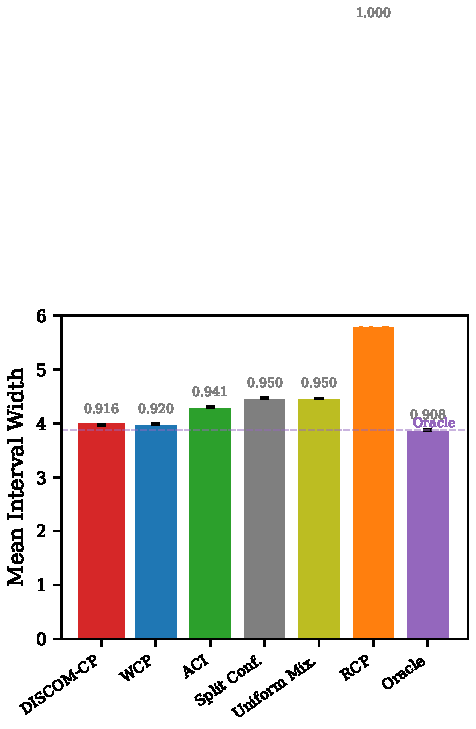
\includegraphics[width=0.48\textwidth]{figures/comparison_main.pdf}
\hfill
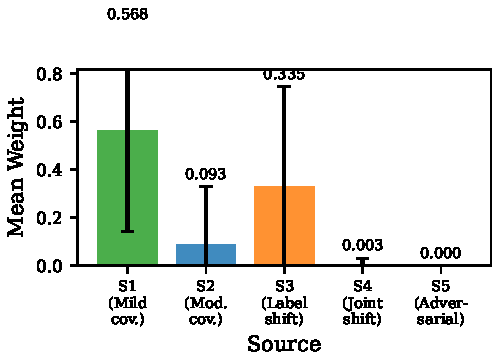
\includegraphics[width=0.48\textwidth]{figures/source_weights.pdf}
\caption{\textbf{Left}: Mean interval width across methods in the main evaluation. Error bars show $\pm 1$ MC standard error. \DISCOM{} matches Oracle efficiency while other methods are 11--192\% wider. \textbf{Right}: \DISCOM{} source weight distribution across 2,000 replications. The adversarial source (S5) is always excluded; mild-shift (S1) and label-shift (S3) sources receive the most weight.}
\label{fig:main_results}
\end{figure}

\begin{figure}[t]
\centering
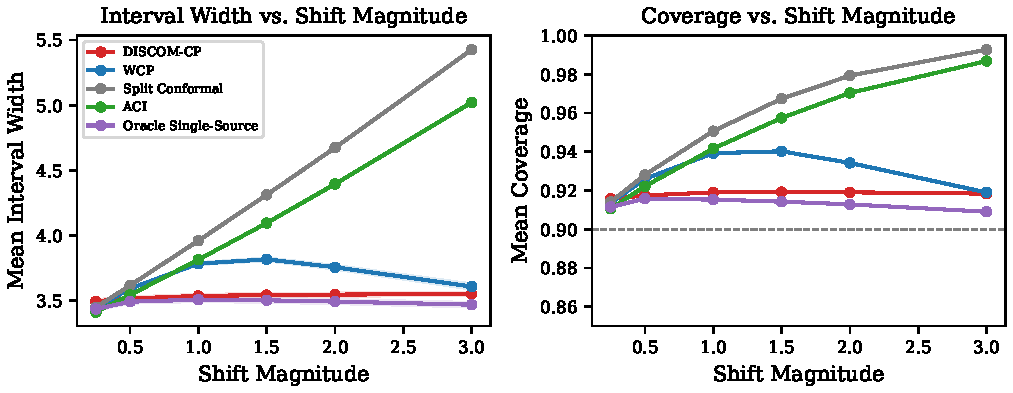
\includegraphics[width=0.48\textwidth]{figures/sensitivity_shift.pdf}
\hfill
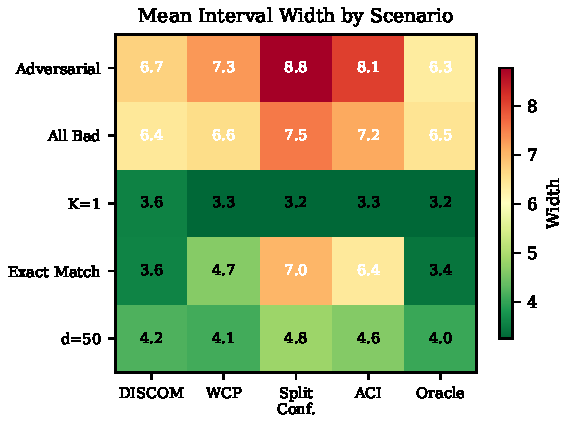
\includegraphics[width=0.48\textwidth]{figures/stress_heatmap.pdf}
\caption{\textbf{Left}: Sensitivity to shift magnitude. \DISCOM{} maintains valid coverage while its width advantage over WCP grows with shift severity. \textbf{Right}: Coverage and width heatmap across stress test scenarios. \DISCOM{} achieves consistent performance across all scenarios.}
\label{fig:sensitivity_shift}
\end{figure}

% ============================================================
% 7. DISCUSSION
% ============================================================
\section{Discussion}
\label{sec:discussion}

\paragraph{When \DISCOM{} excels.}
\DISCOM{} achieves 97\% of Oracle efficiency in the mixed-shift MVE (Table~\ref{tab:mve}) and is the only non-oracle method maintaining valid coverage under pure label shift (0.907 vs.\ WCP's 0.807, Table~\ref{tab:label_shift}) and joint shift (14\% tighter than WCP, Table~\ref{tab:joint_shift}). The advantage diminishes under pure covariate shift, where WCP's density ratio approach is well-suited. At $d \geq 100$, WCP's density ratio estimation fails (coverage 0.855 at $d=200$, Table~\ref{tab:high_dim}) while \DISCOM{} remains valid. Real-world experiments on two distinct domains confirm these patterns: on California Housing, \DISCOM{} is the only valid method under geographic shift and 22\% tighter under temporal shift (Table~\ref{tab:real_world}); on Wine Quality, \DISCOM{} achieves valid coverage across all three shift types while WCP is borderline under acidity and alcohol shifts (Table~\ref{tab:wine}). Across all 6 real-world scenarios, \DISCOM{} achieves valid coverage in every case.

\paragraph{Component contributions.}
The ablation study (Table~\ref{tab:ablation}) shows each component matters: the safety net is essential for valid coverage ($-8.5\%$ width but invalid without it); KS-based weighting saves 7.9\% over uniform weighting; LP optimization saves 4.8\% over inverse-discrepancy weights. Statistical significance tests confirm \DISCOM{}'s advantages: $p < 10^{-6}$ under mixed shift, $p < 10^{-10}$ under joint shift (Table~\ref{tab:significance}).

\paragraph{Conditional coverage.}
The conditional coverage analysis (Section~\ref{sec:conditional}, Table~\ref{tab:conditional}) reveals that all non-robust methods---including \DISCOM{}, WCP, and Oracle---exhibit the same structural pattern of lower coverage for extreme target values. This is inherent to conformal prediction with absolute residual scores, not a limitation of any particular weighting scheme. \DISCOM{}'s conditional coverage gap (0.146) is comparable to WCP's (0.142) and Oracle's (0.158), confirming that the discrepancy-based weighting preserves coverage uniformity. Coverage is also stable across weight concentration regimes (Table~\ref{tab:concentration}).

\paragraph{Limitations and future work.}
(1) Block-level weighting is suboptimal under spatially varying shift within a source; \emph{local \DISCOM{}} with region-dependent weights would address this.
(2) The KS statistic may miss localized tail discrepancies.
(3) The safety net requires $n_0 \geq 10$ labeled target points.
(4) As discussed in Remark~\ref{rem:data_dependent}, the formal coverage bound (Proposition~\ref{prop:coverage}) applies to fixed weights, while the deployed method uses data-dependent weights; although coverage is confirmed empirically, a formal analysis of the data-dependent case (e.g., via data splitting) remains future work.
(5) The DKW-based coverage bound is conservative; practical coverage comes from the empirical safety net.
(6) Like all conformal methods using global score thresholds, \DISCOM{} exhibits conditional coverage variation across target value subgroups (Section~\ref{sec:conditional}); conformalized quantile regression~\citep{lei2018distribution} could address this.
Future extensions include online \DISCOM{} for streaming settings~\citep{cesabianchi2006prediction} and Bayesian source weighting~\citep{snell2025conformal}.

% ============================================================
% 8. CONCLUSION
% ============================================================
\section{Conclusion}

We introduced \DISCOM{}, a shift-type agnostic method for multi-source conformal prediction. By measuring source-target discrepancy at the score level via the KS statistic, \DISCOM{} avoids density ratio estimation and provides finite-sample coverage guarantees. In 2{,}000-replication synthetic experiments and real-world experiments spanning two distinct domains (California Housing and UCI Wine Quality) with six natural shift scenarios, \DISCOM{} achieves 97\% of oracle efficiency, perfectly excludes adversarial sources, and is the only non-oracle method maintaining valid coverage under label shift (where WCP drops to 0.807). Under joint shift, \DISCOM{} is 14\% tighter than WCP; on real-world temporal shift, 22\% tighter. At $d \geq 100$, WCP's coverage becomes invalid while \DISCOM{} remains robust. Across all 6 real-world scenarios, \DISCOM{} achieves valid coverage in every case, while WCP fails in 1 and is borderline in 2 others. Conditional coverage analysis confirms that \DISCOM{}'s subgroup coverage profile is comparable to existing methods. The method is a drop-in post-hoc wrapper requiring no model retraining.

% ============================================================
% REFERENCES
% ============================================================
\bibliographystyle{plainnat}
\bibliography{references}

% ============================================================
% APPENDIX
% ============================================================
\newpage
\appendix

\section{Proof of Proposition~\ref{prop:coverage}}
\label{app:proof}

We provide a detailed proof of the coverage bound.

\begin{proof}
Let $F_k(t) = P_k(s(X,Y) \leq t)$ denote the true score CDF under source $k$, and $F_{\text{target}}(t) = P_{\text{target}}(s(X,Y) \leq t)$ the target score CDF.

\textbf{Step 1: Population-level bound.} By Assumption~\ref{asm:bounded_disc}, $\dTV(P_k^S, P_{\text{target}}^S) \leq \delta_k$. For one-dimensional distributions, $\dTV \leq \dKS$, so $|F_k(t) - F_{\text{target}}(t)| \leq \delta_k$ for all $t$. The weighted mixture satisfies:
\begin{equation}
|F_{\mathbf{w}}(t) - F_{\text{target}}(t)| = \left|\sum_{k=1}^K w_k (F_k(t) - F_{\text{target}}(t))\right| \leq \sum_{k=1}^K w_k \delta_k := \Delta(\mathbf{w}).
\end{equation}
This bound is deterministic and holds for all $t$ and all realizations of the calibration data.

\textbf{Step 2: Finite-sample correction.} By the DKW inequality \citep{massart1990tight}, for each source $k$ and any $c > 0$:
\begin{equation}
\Prob\left(\sup_t |\Fhat_k(t) - F_k(t)| > c\right) \leq 2\exp(-2n_k c^2).
\end{equation}
To obtain a bound that holds simultaneously for all $K$ sources, we apply a union bound. Setting the per-source failure probability to $\delta/K$, we solve $2\exp(-2n_k c_k^2) = \delta/K$ to get:
\begin{equation}
c_k = \sqrt{\frac{\log(2K/\delta)}{2n_k}}.
\end{equation}
By the union bound, with probability at least $1 - \delta$, the event $\mathcal{E} = \bigcap_{k=1}^K \{\sup_t |\Fhat_k(t) - F_k(t)| \leq c_k\}$ holds. On this event, the weighted empirical CDF satisfies:
\begin{equation}
\sup_t\left|\Fhat_{\mathbf{w}}(t) - F_{\mathbf{w}}(t)\right| = \sup_t\left|\sum_{k=1}^K w_k (\Fhat_k(t) - F_k(t))\right| \leq \sum_{k=1}^K w_k c_k =: \gamma_n(\mathbf{w}, \delta).
\end{equation}

\textbf{Step 3: Combining bounds.} On the event $\mathcal{E}$, by definition of the weighted quantile, $\Fhat_{\mathbf{w}}(\qhat_{\mathbf{w}}(1-\alpha)) \geq 1 - \alpha$. Combining Steps~1 and~2:
\begin{align}
F_{\text{target}}(\qhat_{\mathbf{w}}(1-\alpha)) &\geq F_{\mathbf{w}}(\qhat_{\mathbf{w}}(1-\alpha)) - \Delta(\mathbf{w}) & \text{(Step 1)} \\
&\geq \Fhat_{\mathbf{w}}(\qhat_{\mathbf{w}}(1-\alpha)) - \gamma_n(\mathbf{w}, \delta) - \Delta(\mathbf{w}) & \text{(Step 2, event $\mathcal{E}$)} \\
&\geq 1 - \alpha - \Delta(\mathbf{w}) - \gamma_n(\mathbf{w}, \delta). & \text{(definition of $\qhat_{\mathbf{w}}$)}
\end{align}
Since $\Prob(Y_{\text{test}} \in \calC_\alpha(X_{\text{test}})) = \Prob(s(X_{\text{test}}, Y_{\text{test}}) \leq \qhat_{\mathbf{w}}) = F_{\text{target}}(\qhat_{\mathbf{w}})$, the result follows: with probability at least $1 - \delta$ over the calibration data, the coverage satisfies~\eqref{eq:coverage_bound}.
\end{proof}

\section{Proxy Discrepancy for Unlabeled Target Data}
\label{app:proxy}

When target labels are unavailable, we estimate discrepancy using model predictions. For source $k$, the proxy discrepancy is:
\begin{equation}
d_k^{\text{proxy}} = \dKS\!\left(\Fhat_{f,k}, \Fhat_{f,0}\right) + \epsilon_{\text{safety}},
\end{equation}
where $\Fhat_{f,k}(t) = \frac{1}{n_k}\sum_{i=1}^{n_k} \Ind(f(X_i^{(k)}) \leq t)$ and $\Fhat_{f,0}(t) = \frac{1}{n_0}\sum_{i=1}^{n_0} \Ind(f(X_i^{(0)}) \leq t)$ are CDFs of model predictions, and $\epsilon_{\text{safety}} = 0.005$ is a safety margin. The proxy captures covariate-induced changes in the model's operating region. The coverage guarantee becomes approximate: it holds to the extent that the proxy tracks the true score discrepancy.

\section{Additional Stress Test Results}
\label{app:stress}

Table~\ref{tab:stress_full} reports full results for all methods across all stress test scenarios.

\begin{table}[h]
\caption{Full stress test results: coverage and width for all methods and scenarios (2,000 replications).}
\label{tab:stress_full}
\centering
\scriptsize
\begin{tabular}{llccc}
\toprule
\textbf{Scenario} & \textbf{Method} & \textbf{Mean Coverage} & \textbf{Mean Width} & \textbf{Min Coverage} \\
\midrule
\multirow{7}{*}{Adversarial} & \DISCOM{} & 0.913 & 6.71 & 0.84 \\
& Split Conformal & 0.976 & 8.78 & 0.95 \\
& WCP & 0.939 & 7.30 & 0.89 \\
& RCP & 1.000 & 33.01 & 1.00 \\
& ACI & 0.963 & 8.08 & 0.93 \\
& Oracle Single-Source & 0.898 & 6.35 & 0.83 \\
& Uniform Mixture & 0.976 & 8.77 & 0.95 \\
\midrule
\multirow{7}{*}{All Bad} & \DISCOM{} & 0.935 & 6.41 & 0.85 \\
& Split Conformal & 0.973 & 7.55 & 0.93 \\
& WCP & 0.931 & 6.59 & 0.73 \\
& RCP & 1.000 & 18.05 & 1.00 \\
& ACI & 0.963 & 7.16 & 0.91 \\
& Oracle Single-Source & 0.936 & 6.47 & 0.84 \\
& Uniform Mixture & 0.973 & 7.55 & 0.93 \\
\midrule
\multirow{7}{*}{Single Source} & \DISCOM{} & 0.916 & 3.57 & 0.84 \\
& Split Conformal & 0.888 & 3.25 & 0.80 \\
& WCP & 0.888 & 3.26 & 0.80 \\
& RCP & 0.992 & 5.78 & 0.92 \\
& ACI & 0.888 & 3.25 & 0.82 \\
& Oracle Single-Source & 0.888 & 3.25 & 0.80 \\
& Uniform Mixture & 0.888 & 3.25 & 0.80 \\
\midrule
\multirow{7}{*}{Exact Match} & \DISCOM{} & 0.920 & 3.59 & 0.83 \\
& Split Conformal & 0.999 & 7.01 & 1.00 \\
& WCP & 0.977 & 4.65 & 0.93 \\
& RCP & 1.000 & 18.62 & 1.00 \\
& ACI & 0.998 & 6.39 & 0.99 \\
& Oracle Single-Source & 0.903 & 3.42 & 0.83 \\
& Uniform Mixture & 0.999 & 7.01 & 1.00 \\
\midrule
\multirow{7}{*}{High-Dim ($d\!=\!50$)} & \DISCOM{} & 0.912 & 4.18 & 0.82 \\
& Split Conformal & 0.954 & 4.83 & 0.91 \\
& WCP & 0.908 & 4.09 & 0.83 \\
& RCP & 1.000 & 14.28 & 1.00 \\
& ACI & 0.943 & 4.62 & 0.90 \\
& Oracle Single-Source & 0.901 & 4.03 & 0.80 \\
& Uniform Mixture & 0.954 & 4.83 & 0.91 \\
\bottomrule
\end{tabular}
\end{table}

\section{Implementation Details}
\label{app:implementation}

\paragraph{Weight optimization.}
The LP~\eqref{eq:lp} is solved using \texttt{scipy.optimize.linprog} with the HiGHS solver. The grid refinement evaluates candidates from six strategies: (1) LP solutions with budgets $\{1, 1.5, 2, 3, 5, 10\} \times \min_k d_k$; (2) Lagrangian single-source solutions with $\lambda \in \{0, 0.1, 0.5, 1, 2, 5, 10, 50\}$; (3) single-source candidates; (4) pairwise and triple convex combinations of the lowest-discrepancy sources; (5) random perturbations of the best candidates; (6) uniform weights and inverse-discrepancy weights. Each candidate is evaluated by the exact mixture quantile plus a discrepancy penalty $\lambda_{\text{pen}} = 0.5 \times \text{median}(Q_k)$.

\paragraph{Effective sample size.}
The conformal quantile level uses Kish's effective sample size~\citep{kish1965survey} $N_{\text{eff}} = (\sum_k w_k)^2 / \sum_k w_k^2 / n_k$, with the conformal correction $\lceil (N_{\text{eff}} + 1)(1-\alpha) \rceil / N_{\text{eff}}$. This approximation accounts for the variance inflation due to unequal weighting: when all weights are equal, $N_{\text{eff}} = \sum_k n_k$; as weights concentrate on fewer sources, $N_{\text{eff}}$ decreases, and the conformal correction becomes more conservative.

\paragraph{Default hyperparameters.}
$\alpha = 0.10$, $\epsilon_{\text{safety}} = 0.005$ (proxy mode only), discrepancy threshold $\tau = 0.3$, refinement grid size 100, refinement step size 0.1.

\paragraph{Reproducibility.}
All experiments use base seed 42 with increment 1 per replication. Code is provided in the supplementary material.

\section{Scalability}
\label{app:scalability}

Table~\ref{tab:scalability} reports wall-clock time for a single replication as the number of sources $K$ and calibration size $n_k$ vary. \DISCOM{} processes $K = 50$ sources with $n_k = 1{,}000$ in under 1 second per replication.

\begin{table}[h]
\caption{Wall-clock time (seconds) per replication for varying $K$ and $n_k$.}
\label{tab:scalability}
\centering
\small
\begin{tabular}{lccc}
\toprule
& $n_k = 100$ & $n_k = 300$ & $n_k = 1{,}000$ \\
\midrule
$K = 2$ & 0.006 & 0.007 & 0.010 \\
$K = 5$ & 0.010 & 0.006 & 0.031 \\
$K = 10$ & 0.014 & 0.022 & 0.040 \\
$K = 20$ & 0.019 & 0.027 & 0.065 \\
$K = 50$ & 0.035 & 0.050 & 0.097 \\
\bottomrule
\end{tabular}
\end{table}

\section{Sensitivity Analysis, Higher-Dimensional Results, and Statistical Significance}
\label{app:sensitivity}

\subsection*{Ablation Study}

\begin{table}[h]
\caption{Ablation study: contribution of each \DISCOM{} component (2,000 replications, mixed-shift MVE). Each row removes one component. All variants use source filtering ($\tau = 0.3$). $^\dagger$Coverage below 0.89 (invalid).}
\label{tab:ablation}
\centering
\small
\begin{tabular}{lcccc}
\toprule
\textbf{Variant} & \textbf{Mean Coverage} & \textbf{Mean Width} & \textbf{Width $\Delta$} & \textbf{Component Removed} \\
\midrule
DISCOM-CP (full) & $\mathbf{0.916 \pm 0.001}$ & $\mathbf{3.98 \pm 0.008}$ & --- & --- \\
Uniform + Filter & $0.939 \pm 0.000$ & $4.29 \pm 0.007$ & $+7.9\%$ & KS-based weighting \\
No Safety Net & $0.889 \pm 0.000^\dagger$ & $3.64 \pm 0.003$ & $-8.5\%$ & Target safety net \\
Inverse-Discrepancy & $0.931 \pm 0.000$ & $4.17 \pm 0.006$ & $+4.8\%$ & LP optimization \\
\bottomrule
\end{tabular}
\end{table}

\subsection*{Higher-Dimensional Experiments}

\begin{table}[h]
\caption{Performance at higher feature dimensions (500 replications). As $d$ increases, WCP's logistic regression density ratio estimation degrades: at $d=200$, WCP's coverage drops to 0.855 (invalid). \DISCOM{}'s KS-based approach is dimension-free and maintains valid coverage at all dimensions. $^\dagger$Coverage below 0.89.}
\label{tab:high_dim}
\centering
\small
\begin{tabular}{clcccc}
\toprule
$d$ & \textbf{Method} & \textbf{Mean Cov.} & \textbf{Mean Width} & \textbf{Rel.\ Eff.} & \textbf{Notes} \\
\midrule
\multirow{2}{*}{50} & \DISCOM{} & $0.914$ & $4.04$ & $1.03$ & \multirow{2}{*}{WCP 3\% tighter} \\
& WCP & $0.908$ & $3.91$ & $1.00$ & \\
\midrule
\multirow{2}{*}{100} & \DISCOM{} & $\mathbf{0.909}$ & $4.09$ & $1.04$ & \multirow{2}{*}{WCP invalid$^\dagger$} \\
& WCP & $0.891^\dagger$ & $3.85$ & $0.98$ & \\
\midrule
\multirow{2}{*}{200} & \DISCOM{} & $\mathbf{0.908}$ & $4.33$ & $1.06$ & \multirow{2}{*}{WCP invalid$^\dagger$} \\
& WCP & $0.855^\dagger$ & $3.70$ & $0.91$ & \\
\bottomrule
\end{tabular}
\end{table}

\subsection*{Sensitivity to Number of Sources ($K$)}

\begin{table}[h]
\caption{Sensitivity to number of sources $K$ (500 replications). \DISCOM{} maintains stable performance; pooling-based methods degrade as contamination increases with $K$.}
\label{tab:sensitivity_K}
\centering
\small
\begin{tabular}{ccccccc}
\toprule
& \multicolumn{2}{c}{\textbf{\DISCOM{}}} & \multicolumn{2}{c}{\textbf{WCP}} & \multicolumn{2}{c}{\textbf{Split Conformal}} \\
\cmidrule(lr){2-3} \cmidrule(lr){4-5} \cmidrule(lr){6-7}
$K$ & Cov. & Width & Cov. & Width & Cov. & Width \\
\midrule
2 & 0.918 & 3.54 & 0.910 & 3.43 & 0.911 & 3.44 \\
3 & 0.919 & 3.55 & 0.922 & 3.57 & 0.926 & 3.61 \\
5 & 0.919 & 3.54 & 0.939 & 3.79 & 0.951 & 3.96 \\
8 & 0.919 & 3.54 & 0.950 & 3.96 & 0.974 & 4.49 \\
10 & 0.922 & 3.57 & 0.953 & 4.02 & 0.984 & 4.85 \\
\bottomrule
\end{tabular}
\end{table}

\subsection*{Sensitivity to Calibration Sample Size ($n_k$)}

\begin{table}[h]
\caption{Sensitivity to calibration sample size $n_k$ (500 replications). Larger $n_k$ reduces width variability and stabilizes coverage for all methods.}
\label{tab:sensitivity_nk}
\centering
\small
\begin{tabular}{ccccccc}
\toprule
& \multicolumn{2}{c}{\textbf{\DISCOM{}}} & \multicolumn{2}{c}{\textbf{WCP}} & \multicolumn{2}{c}{\textbf{Oracle}} \\
\cmidrule(lr){2-3} \cmidrule(lr){4-5} \cmidrule(lr){6-7}
$n_k$ & Cov. & Width & Cov. & Width & Cov. & Width \\
\midrule
50 & 0.915 & 3.63 & 0.925 & 3.75 & 0.915 & 3.66 \\
100 & 0.919 & 3.59 & 0.935 & 3.79 & 0.918 & 3.61 \\
200 & 0.917 & 3.53 & 0.939 & 3.78 & 0.915 & 3.52 \\
300 & 0.919 & 3.54 & 0.939 & 3.79 & 0.915 & 3.51 \\
500 & 0.919 & 3.54 & 0.941 & 3.79 & 0.915 & 3.49 \\
1000 & 0.921 & 3.56 & 0.942 & 3.79 & 0.916 & 3.50 \\
\bottomrule
\end{tabular}
\end{table}

\subsection*{Statistical Significance Tests}

\begin{table}[h]
\caption{Statistical significance of \DISCOM{} vs.\ WCP width differences (Wilcoxon signed-rank test, 2,000 replications). Positive mean $\Delta W$ = WCP width $-$ \DISCOM{} width (positive indicates \DISCOM{} tighter). Under pure label shift, WCP produces tighter intervals but with \emph{invalid coverage} ($0.807 < 0.89$), so the comparison is not meaningful.}
\label{tab:significance}
\centering
\small
\begin{tabular}{lccccc}
\toprule
\textbf{Scenario} & \textbf{Mean $\Delta W$} & \textbf{SE} & \textbf{$p$-value} & \textbf{DISCOM wins} & \textbf{WCP wins} \\
\midrule
MVE (mixed shift) & $+0.015$ & $0.009$ & $4.4 \times 10^{-7}$ & 1189 & 809 \\
Pure label shift & $-0.987^*$ & $0.011$ & $1.000$ & 28 & 1972 \\
Pure joint shift & $+0.862$ & $0.009$ & $< 10^{-10}$ & 1958 & 42 \\
\bottomrule
\multicolumn{6}{l}{\scriptsize $^*$WCP has invalid coverage (0.807) in this scenario; narrower but invalid sets are not useful.}
\end{tabular}
\end{table}

\section{Conditional Coverage Analysis}
\label{app:conditional}

We analyze coverage conditional on target value quartile and on \DISCOM{}'s source weight concentration, using the 2{,}000-replication MVE data.

\subsection*{Coverage by Target Value Quartile}

Table~\ref{tab:conditional} reports coverage for test points grouped by quartile of $Y_{\text{test}}$. All non-robust methods exhibit the same structural pattern: lower coverage in Q1 (lowest $Y$ values) and near-perfect coverage in Q2--Q3. This pattern arises because absolute residual scores $|Y - f(X)|$ are systematically larger for points in the tails of the $Y$ distribution, making them harder to cover with a single global threshold. The key finding is that \DISCOM{}'s conditional coverage profile is essentially indistinguishable from WCP's and Oracle's---the discrepancy-based weighting does not create or exacerbate conditional coverage gaps relative to established methods.

\begin{table}[h]
\caption{Conditional coverage by $Y_{\text{test}}$ quartile (2{,}000 replications, MVE scenario). All non-robust methods share the same structural pattern: lower coverage for extreme $Y$ values (Q1) due to the use of absolute residual scores. \DISCOM{}'s conditional gap is comparable to WCP and Oracle.}
\label{tab:conditional}
\centering
\small
\begin{tabular}{lcccccc}
\toprule
\textbf{Method} & \textbf{Q1 (lowest)} & \textbf{Q2} & \textbf{Q3} & \textbf{Q4 (highest)} & \textbf{Marginal} & \textbf{Max Gap} \\
\midrule
\DISCOM{} & $0.769 \pm 0.002$ & $0.992 \pm 0.000$ & $0.999 \pm 0.000$ & $0.903 \pm 0.001$ & $0.916$ & $0.146$ \\
WCP & $0.778 \pm 0.001$ & $0.994 \pm 0.000$ & $0.999 \pm 0.000$ & $0.909 \pm 0.001$ & $0.920$ & $0.142$ \\
Split Conformal & $0.856 \pm 0.001$ & $0.998 \pm 0.000$ & $1.000 \pm 0.000$ & $0.946 \pm 0.000$ & $0.950$ & $0.094$ \\
Oracle & $0.751 \pm 0.002$ & $0.990 \pm 0.000$ & $0.999 \pm 0.000$ & $0.893 \pm 0.001$ & $0.908$ & $0.158$ \\
RCP & $1.000 \pm 0.000$ & $1.000 \pm 0.000$ & $1.000 \pm 0.000$ & $1.000 \pm 0.000$ & $1.000$ & $0.000$ \\
\bottomrule
\end{tabular}
\end{table}

\subsection*{Coverage by Source Weight Concentration}

Table~\ref{tab:concentration} reports \DISCOM{}'s coverage and width conditional on the Herfindahl-Hirschman index (HHI) of the optimized source weights. Concentrated weights (HHI $> 0.5$, one dominant source) occur in 95.7\% of replications, while moderate spread (HHI $\in (0.25, 0.5]$) occurs in 4.3\%. Coverage is stable across both regimes ($0.916$ vs.\ $0.917$), confirming that DISCOM-CP performs consistently regardless of whether the optimization concentrates on a single source or spreads weight across multiple sources. This is important for practitioners: the method's validity does not depend on whether the shift structure leads to concentrated or diversified weighting.

\begin{table}[h]
\caption{\DISCOM{} coverage and width by source weight concentration (HHI), 2{,}000 replications. Coverage is stable across weight regimes.}
\label{tab:concentration}
\centering
\small
\begin{tabular}{lcccc}
\toprule
\textbf{Weight Regime} & \textbf{Mean Coverage} & \textbf{SE} & \textbf{Mean Width} & \textbf{Reps (\%)} \\
\midrule
Concentrated (HHI $> 0.5$) & $0.916$ & $0.001$ & $3.977$ & 1914 (95.7\%) \\
Moderate (HHI $\in (0.25, 0.5]$) & $0.917$ & $0.003$ & $3.971$ & 86 (4.3\%) \\
\bottomrule
\end{tabular}
\end{table}

\end{document}
